\documentclass{article}
\usepackage{amsmath, amssymb, amsthm}
\usepackage{tikz}
\usepackage{geometry}
\usepackage[T1]{fontenc}
\geometry{margin=1in}

\title{MAIA 1: Topologie i przestrzenie metryczne}
\author{}
\date{}

\begin{document}
\maketitle

\section{Podstawowa terminologia}

\subsection{Zbiory i rodziny}

\begin{enumerate}

\item przestrzeń/zbiór -- $X$
\item podzbiór -- $A \subseteq X$
\item dopełnienie podzbioru -- $A^c = \{x \in X : x \notin A\}$
\item zbiór pusty -- $\emptyset = X^c$
\item zbiór potęgowy / wszystkich podzbiorów -- $\mathcal{P}(X)$ lub $2^X$ ($A^B$ to ogólnie wszystkie funkcje $f: B \to A$)
\item rodzina podzbiorów -- $\mathcal{F}(X) \subseteq \mathcal{P}$

\end{enumerate}


\subsection{Złożenia zbiorów}

\begin{enumerate}

\item dla $A_\alpha \subset X$ gdzie $\alpha \in I$ (dowolny zbiór indeksów)

$$\bigcup_{\alpha \in I} A_\alpha = \{x \in X: \exists_{\alpha\in I}(x \in A_\alpha)\}$$

$$\bigcap_{\alpha \in I} A_\alpha = \{x \in X: \forall_{\alpha \in\ I}(x \in A_\alpha)\}$$

\item dla $A_n \subset X$ gdzie $n \in \mathbb{N}$

$$\limsup_{n \to \infty} A_n = \bigcap_{n=1}^{\infty} \left( \bigcup_{k \geq n} A_k \right)$$

$$\liminf_{n \to \infty} A_n = \bigcup_{n=1}^{\infty} \left( \bigcap_{k \geq n} A_k \right)$$

\textbf{fakt:} $\liminf A_n \subseteq \limsup A_n$

\textbf{fakt:} $\left( \liminf A_n \right)^c = \left( \limsup A_n\right)^c$

\textbf{fakt:} $\left( \limsup A_n \right)^c = \left( \liminf A_n\right)^c$

$\textbf{def:} \liminf A_n = \limsup A_n \Rightarrow \lim A_n = \liminf A_n = \limsup A_n$

\item iloczyn Kartezjański -- $A \times B = \{(x,y): x \in A, y \in B \}$

\end{enumerate}

\section{Topologie i metryki}

\subsection{Funkcje ciągłe}

\begin{enumerate}
\item funkcja mapująca pomiędzy dwoma przestrzeniami topologicznymi $(X, \tau_1)$ i $(Y, \tau_2)$
\item funkcja odwrotna $f^{-1}[A] = \{x \in X: f(x) \in A\}$
\item funkcja $f$ jest ciągła iff $\forall_{A \in \tau_2} f^{-1}[A] \in \tau_1$
\end{enumerate}

\subsection{Przestrzeń metryczna}

funkcja $d$ jest metryką na $X$ jeśli $d: X \times X \to [0,\infty)$ i spełnia warunki

\begin{enumerate}
\item odległość punktu do siebie jest zerem, $\forall_{x, y \in X} \mkern5mu d(x,y) = 0 \Leftrightarrow x = y $
\item jest symetryczna, $\forall_{x, y \in X} \mkern5mu d(x,y) = d(y,x)$
\item nierówność trójkąta, $\forall_{x, y, z \in X} \mkern5mu d(x,y) \leq d(x,z) + d(z,y)$
\end{enumerate}

\subsection{Kula}

dla $x_0 \in X$ i $R > 0$ kulą jest zbiór

$$B(x_0, R) = \{x \in X: d(x_0, x) < R\}$$

\subsection{Zbióry otwatre i zamknięte}

\begin{enumerate}

\item $A \subset X$ jest otwarty w $X$ jeśli mieści się w kulim czyli

$$\forall_{x \in A} \exists_{R > 0} B(x, R) \subset A$$

\item przykład dla $X = \mathbb{R}^2$ może być

$$d_0\left((x_1,y_1), (x_2,y_2)\right) = \begin{cases} 
0 & \text{if } (x_1,y_1) = (x_2,y_2) \\
1 & \text{otherwise}
\end{cases}$$
i potem $d_1$ (Manhattan distance) i $d_2$ (Euclidean)

\item dopełnieniem zbioru otwartego nazywamy zbiorem zamkniętym

\textbf{fakt:} dopełnienie kuli to sfera (powierzchnia)

\end{enumerate}

\subsection{Przestrzeń topologiczna}

Rodzina podzbiorów $\tau$ jest topologią na zbiorze $X$ gdy dla wszystkich otwartych zbiorów $A \in \tau$,

\begin{enumerate}
\item dowolna unia jest zawarta: $A_\alpha \in \tau, \; \alpha \in I \Rightarrow \bigcup_{\alpha \in I} A_\alpha \in \tau$
\item dowolny przekrój jest zawarta: $A_\alpha \in \tau, \; \alpha \in I \Rightarrow \bigcap_{k=1}^n A_k \in \tau$
\item $\emptyset, X \in \tau$
\end{enumerate}

\section{Przestrzenie liniowe i unormowane}

\begin{enumerate}
\item ciało $\mathbb{K}$ jest zbiorem na którym suma, róźnica, iloczyn i anty-iloczyn są zdefiniowane
\item przestrzeń liniowa dodatkowo spełnia $\forall_{x,y \in X} \forall_{\alpha,\beta \in X} \alpha x + \beta y \in X$
\item przestrzeń unormowana dodatkowo definiuje normę $(X, \|\cdot\|) \rightarrow \|\cdot\|: X \to [0,\infty)$ gdzie
\begin{enumerate}
\item norma jest zerowa tylko dla zera, $\|x\| = 0 \Leftrightarrow x = 0$
\item absolute homogeneity, $\forall_{x \in X} \forall_{\alpha \in \mathbb{K}} \|\alpha x\| = |\alpha| \cdot \|x\|$
\item nierówność trójkąta, $\forall_{x,y \in X} \|x+y\| \leq \|x\| + \|y\|$
\end{enumerate}

\textbf{fakt:} odległość zdefiniowana jako $d(x,y) = \|x-y\|$ jest metryką na $X$ (norm induced metric)

\item dla $X = \mathbb{R}^n$ i $\mathbf{x} = (x_1, \ldots, x_n)$ mamy standardowe normy bezwzględne i Euklidesowe i ich uogólnienie,

$$\|\mathbf{x}\|_1 = \sum_{i=1}^{n} |x_i|$$

$$\|\mathbf{x}\|_2 = \sqrt{\sum_{i=1}^{n} x_i^2}$$

$$L_p = \|\mathbf{x}\|_p = \left(\sum_{i=1}^{n} x_i^p\right)^{1/p} \quad (p \geq 1)$$
\item w granicy $L_p$ staje się normę maksymalną

$$L_\infty = \lim_{p \rightarrow \infty} L_p = \max\lbrace |x_1|, |x_2|, ..., |x_n| \rbrace$$

\item dla nieskończonych wektorów (sekwencji) podobnie używając zbioru indeksującego $I$ można zdefiniować normę zbieżną i jej normę maksymalną (to się nazywa przestrzenią Banacha),

$$\ell_p(I) = \{ x = (x_n)_{n \in I}  \in \mathbb{K}: \sum_{n \in I} |x_n|^p < \infty \}$$

$$\ell_\infty = \lim_{p \rightarrow \infty} \ell_p = \sup_{n \in \mathbb{N}} |x_n|$$
\end{enumerate}

\subsection{Przestrzenie unitarne (inner product space)}

\begin{enumerate}
\item przestrzeń liniowa $(X, \langle \cdot, \cdot \rangle)$ na liczbach rzeczywistych lub zespolonych
\item iloczyn wewnętrzny $\langle \cdot, \cdot \rangle: X \times X \to \mathbb{K}$ spełnia warunki:
\begin{enumerate}
\item symetria sprzężona, $\forall_{x,y \in X} \langle x,y \rangle = \overline{\langle y, x \rangle}$
\item limiowość, $\forall_{y_1, y_2,\alpha,\beta,z} \langle \alpha x + \beta y_1, z \rangle = \alpha \langle x, z \rangle + \beta \langle y_1, z \rangle$
\item niezerowość, $\forall_{x \in X, x \neq 0} \langle x, x \rangle > 0$ (lub $\Rightarrow \langle x, x \rangle = 0 \Leftrightarrow x = 0$)
\end{enumerate}
\end{enumerate}

\textbf{fakt:} $\|x\| = \sqrt{\langle x, x \rangle}$ is a norm

\textbf{przykład:} $X = \mathbb{R}^n, \langle x, y \rangle = \sum x_i \cdot y_i$

\begin{center}
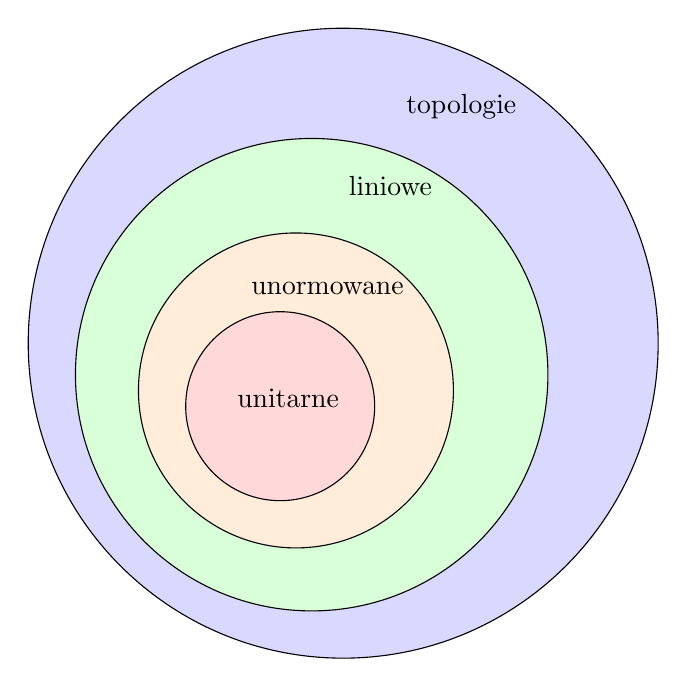
\begin{tikzpicture}
\filldraw[fill=blue!15] (0,0) circle (4cm);
\filldraw[fill=green!15] (-0.4,-0.4) circle (3cm);
\filldraw[fill=orange!15] (-0.6, -0.6) circle (2cm);
\filldraw[fill=red!15] (-0.8,-0.8) circle (1.2cm);
\node at (-0.7,-0.7) {unitarne};
\node at (-0.2,0.7) {unormowane};
\node at (0.6,2) {liniowe};
\node at (1.5,3) {topologie};
\end{tikzpicture}
\end{center}

\subsection{Dalsze przesztrzenia}

\begin{enumerate}
\item ciąg Cauhy'ego na przestrzeni metrycznej, $\forall_{\varepsilon > 0} \exists_N \forall{m,n>N} d(x_n,x_m) < \varepsilon$
\item przestrzeń zupełna (complete, Cauchy), każdy ciąg Cauchy'ego ma zawartą granicę
\item przestrzeń Banacha, zupełna unormowana przestrzeń wektorowa
\item przestrzeń Hilberta, Banacha plus iloczyn wewnętrzny
\end{enumerate}

\subsection{Własności metryki przestrzeni}
\begin{enumerate}
\item nierówność Cauchy'ego-Schwarza,

$$\forall_{x,y \in X} |\langle x,y \rangle| \leq \|x\| \cdot \|y\|$$
or
$$\forall_{x,y \in X} \frac{\langle x,y \rangle}{\|x\| \cdot \|y\|} \in [-1,1]$$

\item twierdzenie Pitagorasa, $x \perp y \iff \|x+y\|^2 = \|x\|^2 + \|y\|^2$, i uogólnienie

$$\|\sum x_k\|^2 = \sum \|x_k\|^2$$

\item kąt pomiędzy wektorami, $\angle(x,y) = \arccos\left(\frac{\langle x,y \rangle}{\|x\| \cdot \|y\|}\right)$
\end{enumerate}

\end{document}
